%% ---------------------------------------------- Chapter Introduction

People need to connect other people, and the urge for connection, bring to us what today are known as \glspl{osn}.
This web sites allows to define a profile as an individual, and to share and visualize content with other individuals in the network, therefore connecting.

\begin{quote}
\textit{"We define Online Social Networks as web-based services that allow individuals to construct a public or semi-public
 profile within a bounded system, articulate a list of other users with whom they share a connection, and view and traverse
 their list of connections and those made by others within the system. The nature and nomenclature of these connections
 may vary from site to site.} \cite{ellison2007social} \footnote{A table is presented on the next page. The blank space is due to the size of the table.}
\end{quote}

%% -------------------------------------------------------------------------------------------- TABLE
\begin{table}[H]
\hspace*{-1.22in}
\renewcommand{\tabcolsep}{2pt}
\begin{tabular}{ |c|c|c|c|l|  }
\hline
\textbf{Name} & \textbf{Year of launch} & \textbf{Registered Users} & \textbf{Provides an API?} & \textbf{Description/Purpose}\\
\hline
\cellcolor{gray!60}Facebook & 2004 & 1 712 000 000 & Yes & \textbf{General}. Photos, videos, blogs, apps.\\
\hline
\cellcolor{gray!60}Google+ & 2011 & 1 600 000 000 & Yes & \begin{tabular}{@{}l@{}}\textbf{General}. Google+ is an interest-based\\social network that is owned\\and operated by Google.\end{tabular}\\
\hline
\cellcolor{gray!60}Youtube & 2005 & 1 000 000 000 & Yes & \begin{tabular}{@{}l@{}}Allows billions of people to discover,\\watch and share originally-created videos.\\Provides a forum for people to connect,\\ inform, and inspire others.\end{tabular}\\
\hline
\cellcolor{gray!30}Qzone & 2005 & 652 000 000 & \textcolor{red}{No} & \begin{tabular}{@{}l@{}}\textbf{General}. It allows users to write blogs,\\keep diaries, send photos, listen to music,\\and watch videos.\\It's only available in Chinese.\end{tabular}\\
\hline
\cellcolor{gray!30}Twitter & 2006 & 645 750 000 & Yes & \textbf{General}. Micro-blogging, RSS, updates.\\
\hline
\cellcolor{gray!30}Tumblr & 2007 & 555 000 000 & Yes & \begin{tabular}{@{}l@{}}Microblogging platform and social\\networking website.\end{tabular}\\
\hline
\cellcolor{gray!30}Instagram & 2010 & 300 000 000 & Yes & A photo and video sharing site.\\
\hline
\cellcolor{gray!30}Sina Weibo & 2009 & 300 000 000 & Yes & \begin{tabular}{@{}l@{}}Social microblogging site in mainland China.\end{tabular}\\
\hline
\cellcolor{gray!30}VK & 2006 & 249 409 900 & Yes & \begin{tabular}{@{}l@{}}\textbf{General}, including music upload, listening\\ and search.\\Popular in Russia and former Soviet republics.\end{tabular} \\
\hline
\cellcolor{gray!30}LinkedIn & 2003 & 200 000 000 & Yes & Business and professional networking.\\
\hline
\cellcolor{gray!30}Vine & \textbf{2013} & 200 000 000 & \textcolor{red}{No} & \begin{tabular}{@{}l@{}}Short-form video sharing service where\\ users can share six-second-long\\looping video clips.\end{tabular}\\
\hline
\cellcolor{gray!30}Pinterest & 2010 & 176 000 000 & Yes & \begin{tabular}{@{}l@{}}The world’s catalog of ideas. Find and save\\recipes, parenting hacks, style inspiration and\\other ideas to try.\end{tabular}\\
\hline
\cellcolor{gray!10}Reddit & 2005 & 35 000 000 & Yes & \begin{tabular}{@{}l@{}}Social media, social news aggregation, web\\content rating, and discussion website.\end{tabular}\\
\hline
\cellcolor{gray!10}Flickr & 2007 & 32 000 000 & Yes & \begin{tabular}{@{}l@{}}Helping people make their photos\\ available to the people who matter to them.\\Enable new ways of organising\\photos and video.\end{tabular}\\
\hline
\cellcolor{gray!10}Meetup & \textbf{2002} & 27 590 000 & Yes & \begin{tabular}{@{}l@{}}World's largest network of local groups.\\Meetup makes it easy for anyone\\to organize a local group or find\\one of the thousands already meeting\\up face-to-face. \cite{meetup}\end{tabular}\\
\hline
\cellcolor{gray!10}Couchsurfing & 2004 & 12 000 000 & \textcolor{red}{No} & \begin{tabular}{@{}l@{}}Couchsurfing connects travellers with\\a global network of people willing\\to share in profound and meaningful ways,\\ making travel a truly\\ social experience. Is commonly used by travellers\\to find free hosts across the globe.\\\cite{csurf}\end{tabular}\\
\hline
\cellcolor{gray!10}ResearchGate & 2008 & 10 000 000 & \textcolor{red}{No} & \begin{tabular}{@{}l@{}}Built by scientists, for scientists.\\Connect the world of\\ science and make\\ research open to all. \cite{rgate}\end{tabular}\\
\hline
\end{tabular}
\caption{\label{table:osns} Table of \glspl{osn} (\cite{statista}, \cite{expandedramblings})}
\end{table}
%% -------------------------------------------------------------------------------------------- TABLE

\indent The Table \ref{table:osns} lists the most used and popular \glspl{osn}, ordered by the estimated number of registered users.
\\\\
\indent The first obvious comment on the listed \glspl{osn} is that general purpose \glspl{osn} have more users (social
networks with the word \textit{General} in bold), being Youtube an exception, since it is not a general purpose \glspl{osn}, neither
is focused on individuals, it is build around \textbf{social objects}, the videos.
\\\\
\indent The grey scale in the first column of Table \ref{table:osns} divides \glspl{osn} in three groups: the first and smallest, the 1 billion
or more users \glspl{osn}; the second the \glspl{osn} with less than 1 billion users and more then 100 million; finally, the third group, \glspl{osn} with
less then 100 million users. At this point, we begin to observe that \textbf{the narrower purpose \glspl{osn}} such as ResearchGate (mainly for researchers) or
Couchsurfing (mainly for open minded travellers), \textbf{have a smaller number of registered users}, which is expected since the target audience is also smaller.
\\\\
\indent Other \glspl{osn} not listed in the Table \ref{table:osns}, but still worth mentioning include \textbf{Classmates} (helps users finding
classmates form kindergarten, primary school, high school etc.) known for being one of the first \glspl{osn}, since it was
launched in 1995, and \textbf{Ask.fm} (allows users to interact with other users asking and answering questions (revealing identity is optional)).


%% ---------------------------------------------- Portuguese and Online Social Networks
\section{Portuguese and Online Social Networks}
From Table \ref{table:osns}, we get a good overview on \glspl{osn} usage among modern society. In this section we do a deep exploration of the most adopted \glspl{osn} by portuguese citizens,
and get to compare then with the more global scenario presented in Table \ref{table:osns}, also, other interesting facts will be revealed where appropriate.\\
\indent A recent study, \cite{marktest2016}, revels portuguese relationship with \glspl{osn}. This study, has been made by \textit{Marktest Consulting} since 2011, with the goal of know the notoriety, utilization, opinion
and habits of portuguese concerning social networks. The study information was collected trough online interviews. The sample was built from 819 interviews from individuals with age between
15 and 64 years, living in Portugal and using \glspl{osn} in a daily basis.\\
\indent Some of the most interesting facts revealed in this study, relative to the participants are:
\begin{itemize}
  \item 94\% has a Facebook account and 43\% a Youtube account;
  \item 21\% has abandoned a social network in the past year;
  \item 27\% considers that their dedicated time to social media has increased;
  \item 67\% follows celebrities and 62\% follows brands;
  \item 87\% is used to watch videos in social networks.
\end{itemize}

\indent These are indeed interesting conclusions, but what about the top used \glspl{osn}, when it comes to that, the most used are the following: 97.2\% uses Facebook; 58.3\% uses Twitter; 54.9\% uses Instagram; 28\% uses LinkedIn;
17.3\% uses Snapchat.\\
\indent Relatively to \cite{marktest2016} past studies, there is one change only, that is the \textbf{ascendence of Instagram to the second most used \glspl{osn}}, Facebook has maintain
its top position, maintaining a grow tendency that has been standing out in the past years.

\indent Going back to Table \ref{table:osns}, we may now comment the portuguese \glspl{osn} comparing it
to the global scenario. As one may notice Facebook still rules users preferences within portuguese.
The other noticeable point is that the \glspl{osn} preferred among portuguese are general propose ones,
but with a slight tendency to content sharing networks (mainly photos), thus, Instagram assuming
a so relevant position in the portuguese landscape.

\indent Concerning to global time related usage statistics, according to \cite{marktest2016}, \textbf{portuguese spend 91 minutes a day with social networks},
68\% considers that this is the ideal time to spent with social media, despite 1 in each 4 saying that in the past year has dedicated even more time to them.
Even if people spent more than one hour and an half in this platforms, the study,
 concluded that \textbf{67\% of the users that visit \glspl{osn} several times a day only 41\% does daily publications}.

\indent \textbf{The prime time for using \glspl{osn} is between 8pm and 10pm}, being the smartphone the most used device in this time. Also in this short period the
featured \gls{osn} is Facebook, the majority of the interviewed say that is the most credible site, the one that provides better and useful information,
the most interesting and addictive.


%% ---------------------------------------------- History of Online Social Networks
\section{History of Online Social Networks}
\begin{figure}[h!]
\begin{center}
  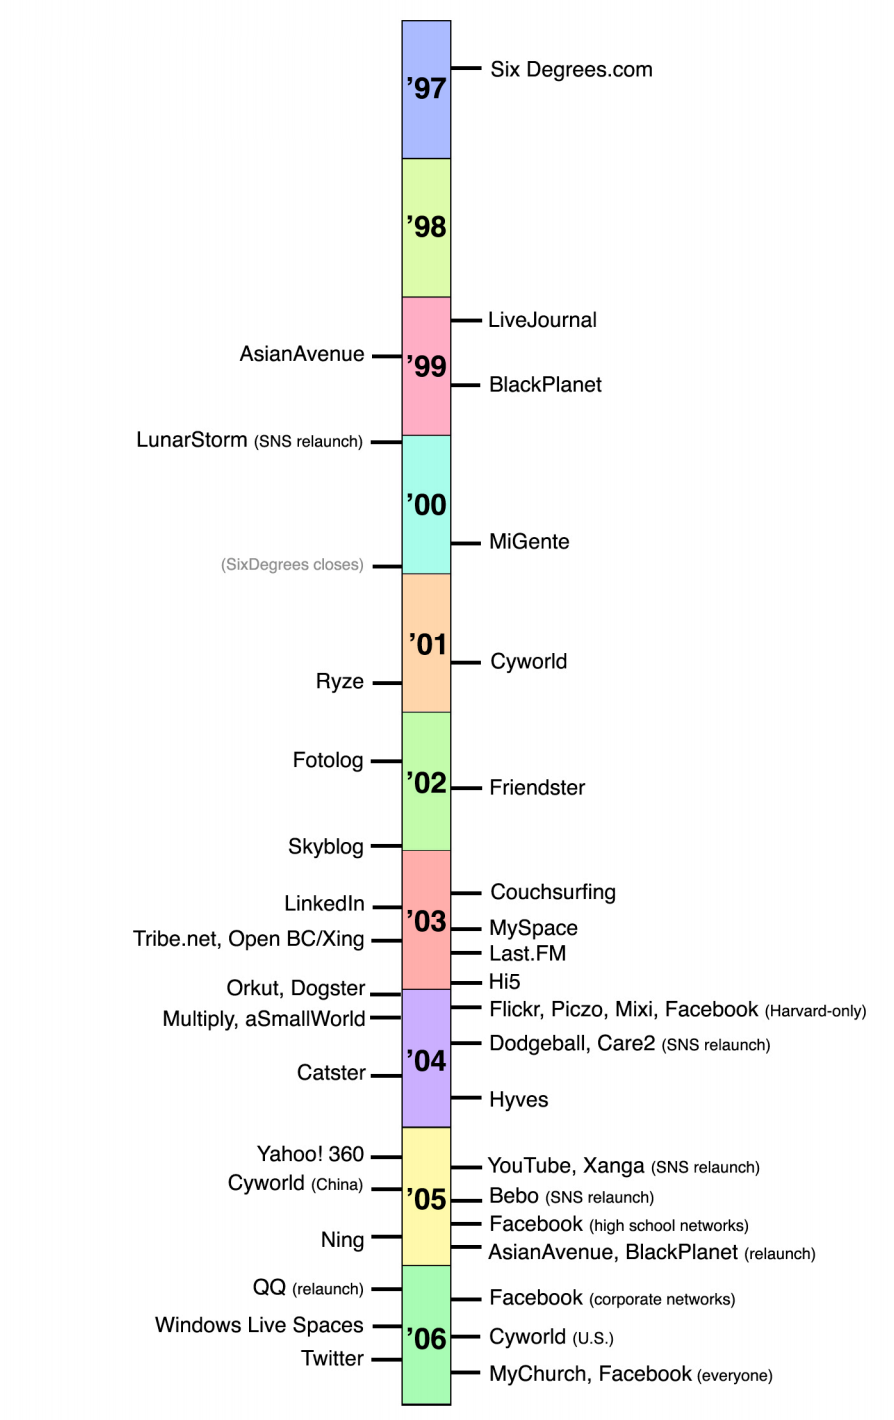
\includegraphics[width=0.7\textwidth]{img/timeline.png}
\end{center}
\caption{\label{img:timeline} Lauch dates of major \glspl{osn}. (\cite{ellison2007social})}
\end{figure}

Although the first platform possessing some of the main characteristics that define \glspl{osn},
according to \cite{ellison2007social}, the first recognizable \gls{osn} launched in 1997 as we can observe in the Figure \ref{img:timeline}. \textit{SixDegrees.com} allowed users to create personal
profiles, connect with friends and consult friends of friends lists. The profile feature came from the
online dating sites and online communities, while the surfing trough register users in the network
and consult friends was an existing feature in Classmates.com. \textit{SixDegrees.com} was the first to combine
these features.

\textit{SixDegrees} promoted itself as a tool to help people to connect, but in 2000, it became an
unsustainable business and the service closed. At the time the creators conclude that
\textit{SixDegrees} was a service that was very ahead of its time.

Until 2002 many \glspl{osn} have emerged, but still incapable of projecting themselves at a global scale.
As we can observe in the timeline of Figure \ref{img:timeline} from 2002 and 2005 the \textit{big players} came to existence, in these period, \gls{osn}
such as Friendster, LinkedIn, MySpace, Hi5, Facebook and Youtube were born, shaping the business, cultural
and research landscape.


%% ---------------------------------------------- Exploring Some OSNs
\section{Exploring Specific Online Social Networks}

In this section we are going to explore in greater detail some of the \glspl{osn} presented
in the Table \ref{table:osns}. The selection of the social networks was not aleatory, we are going
to study deeply the \glspl{osn} that gather some important characteristics, that will be of use in
the future when we design the system for analyzing and visualizing social networks. First, the
\gls{osn} must be accessible, this said, one must be capable of extracting information from the platform
in order to analyze it. Second, in order to obtain large networks, and since this project is being
developed in Portugal, \glspl{osn} that are known to be massively adopted by portuguese (this topic was
addressed in the previous section, where we did an overview to \cite{marktest2016}). Third and at last,
the \glspl{osn} must be the most diversified as possible in terms of their porposes, so that we
can draw different types of conclusions derived from different kind of analysis, for then give proof
of the adaptability of the system to different kinds of \glspl{osn}.\\
\indent This said, these are the following \glspl{osn} that will explored deeply in the proceeding sections:
\begin{itemize}
  \item Facebook
  \item Twitter
  \item LinkedIn
  \item ...
\end{itemize}

\subsection{Facebook}

Facebook allows you to send messages and post status updates to keep in touch with friends and family. You can also share different types
of content, like photos and links. But sharing something on Facebook is a bit different from other types of online communication, because shared content
on facebook is, by default, public.

\subsubsection*{Domain Model}

\begin{figure}[h!]
  \hspace*{-1in}
  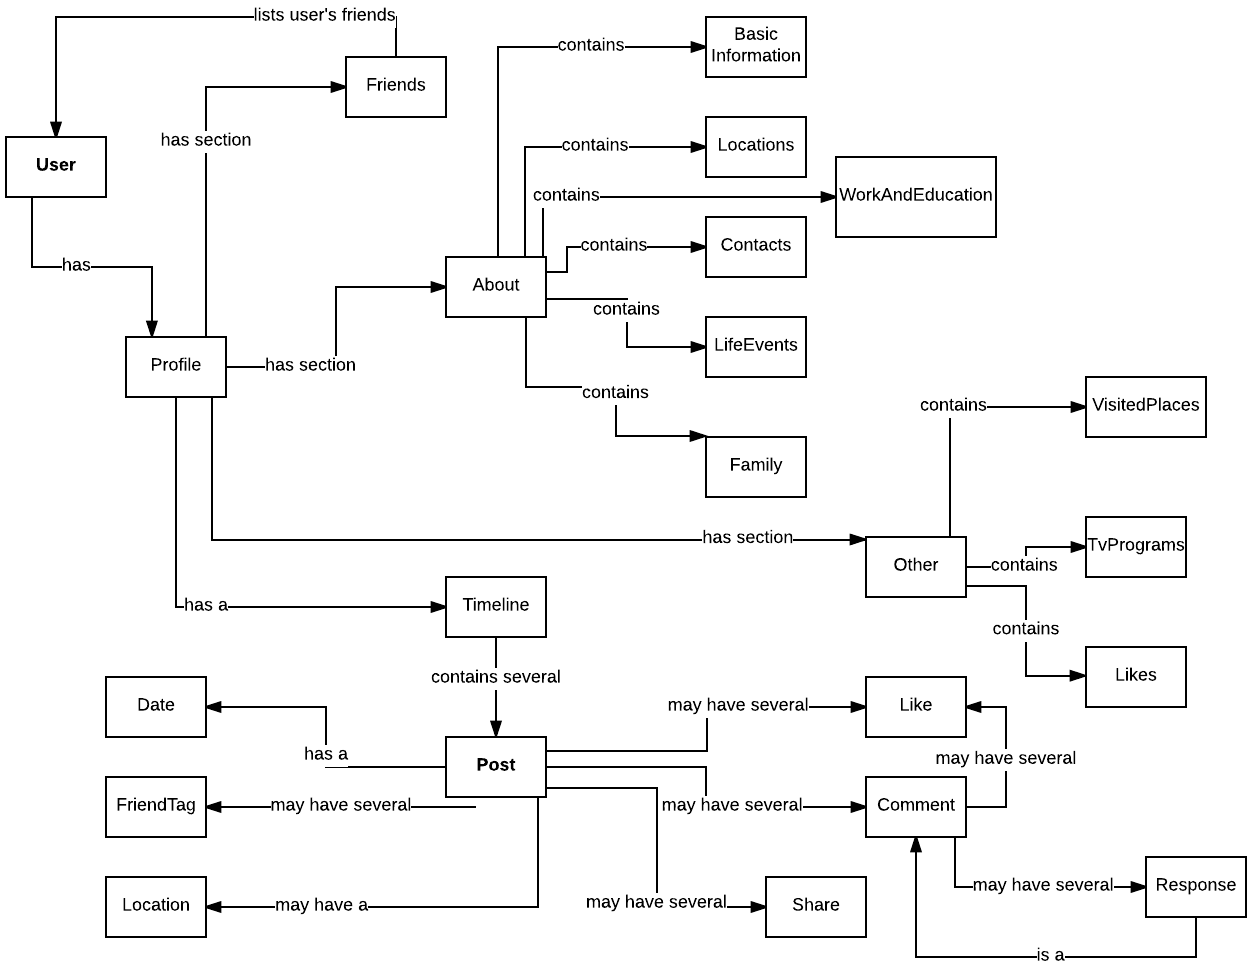
\includegraphics[width=1.2\textwidth]{img/facebook-domain-model.png}
\caption{\label{img:fbdomain} Facebook domain model schema.}
\end{figure}

\indent

\subsubsection*{Facebook Graph API}


%% ---------------------------------------------- How Social Networks Have Changed The World
\section{How Social Networks Have Changed The World}
% Cool overview: https://www.youtube.com/watch?v=trH4iuebjjI
% What really changed? What people did that was good that people don't do anymore? A general overview to the impacts of OSNs!
